\documentclass[tikz,border=4pt]{standalone}
\usepackage{amsmath,amssymb}

\usetikzlibrary{arrows.meta,positioning,automata,shapes,shapes.misc,calc,decorations.pathmorphing,decorations.markings,angles,quotes,patterns,mindmap,matrix,knots,hobby,trees}
\tikzset{->-/.style={decoration={markings, mark=at position 0.5 with {\arrow{Stealth}}}, postaction={decorate}}}
\begin{document}
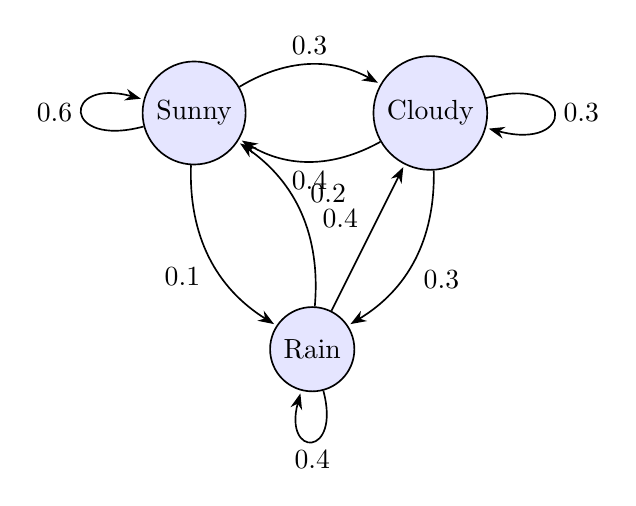
\begin{tikzpicture}[->, >=Stealth, shorten >=1pt, auto, node distance=3cm, semithick, s/.style={circle, draw, fill=blue!10, minimum size=10mm}]
\node[s] (A) {Sunny}; \node[s] (B) [right of=A] {Cloudy}; \node[s] (C) [below of=A, xshift=1.5cm] {Rain};
\path (A) edge [loop left] node {0.6} (A) edge [bend left] node {0.3} (B) edge [bend right] node[swap] {0.1} (C)
      (B) edge [bend left] node {0.4} (A) edge [loop right] node {0.3} (B) edge [bend left] node {0.3} (C)
      (C) edge [bend right] node[swap] {0.2} (A) edge node {0.4} (B) edge [loop below] node {0.4} (C);
\end{tikzpicture}
\end{document}
